\documentclass[letterpaper, 10 pt, conference, twoside]{ieeetran}
%this line out if you need a4paper
%\documentclass[a4paper, 10pt, conference]{ieeeconf}      % Use this line for a4 paper
\IEEEoverridecommandlockouts                              % This command is only needed if 
                                                          % you want to use the \thanks command

%\overrideIEEEmargins                                      % Needed to meet printer requirements.

 
%\usepackage{graphics}
\usepackage{stfloats}
\usepackage[utf8]{inputenc}
\usepackage{graphicx} 
\usepackage{color}
\usepackage{comment}
\usepackage{amssymb,amsmath}
\usepackage{multirow}
\usepackage{float}
\usepackage{bm}
\usepackage{cancel}
\usepackage[dvipsnames]{xcolor}
\usepackage{cite}
\usepackage{booktabs}
\usepackage[hidelinks]{hyperref}
\usepackage[absolute,overlay]{textpos} % For copyright
\usepackage{algorithm}
\usepackage[noend]{algpseudocode}
\usepackage{pgfplots}
\usepgfplotslibrary{groupplots}
\pgfplotsset{compat=1.18}
%\usepackage[top=2.54cm, bottom=2.1cm, left=1.91cm, right=1.91cm]{geometry}
%geometry{top=1.5cm, bottom=1.52cm, left=1.69cm, right=1.69cm}



\title{\LARGE \bf
Reconfigurable Microspine-Enhanced Soft Grippers\\for Extraterrestrial and Martian Rock Grasping}

%\author{,  and Salua Hamaza
\author{Josh van't Sant$^{1}$, Fernando Ruiz$^{1}$, Sebastiaan de Vet$^{2}$ and Salua Hamaza$^{1}$
\thanks{$^{1}$\href{https://www.tudelft.nl/en/ai/biomorphic-intelligence-lab}{Biomorphic Intelligence Lab}, Department of Control \& Operations, TU Delft Aerospace Engineering, The Netherlands. }
\thanks{$^{2}$Planetary Exploration, Department of Space Engineering, TU Delft Aerospace Engineering, The Netherlands.}
}%



\begin{document}
\maketitle
%%%%%%%%%%%%%%%%%%%%%%%%%%%%%%%%%%%%%%%%%%%%%%%%%%%%%%%%%%%%%%%%%%%%%%%%%%%%%%%%
\begin{abstract}

Future planetary exploration platforms could extend the reach of Mars missions by accessing steep, fragmented, or otherwise unreachable terrains, but robust physical interaction with natural surfaces remains a key limitation for sample acquisition and safe touchdown. This paper presents a soft robotic gripper with modular, magnetic snap-fit soft microspine modules as a reconfigurable add-on end-effector compatible with aerial, rover-mounted, and legged platforms. The soft compliant backing of each module simultaneously improves distributed contact with rock asperities and enables tool-free swap of spine morphology, supporting both opportunistic rock grasping and terrain-adaptive landing from a single compliant structure. We experimentally evaluate multiple configurations — varying spine thickness, number, and spatial distribution — through qualitative grasping trials, grasp success rate, and static shear and pull-off force measurements across four Mars-relevant rock analogues. Results show that thick-spine configurations provide superior engagement on coarse-grained, high-asperity surfaces, while thin-spine configurations achieve higher success rates on fine-grained or smoother rocks. These relationships are used to propose a terrain-compatibility framework linking microspine morphology to Martian geological context, providing design guidelines for end-effectors reconfigurable to match surface conditions at a target exploration site.

\textit{Index Terms:} Microspines, Soft Robotics, Planetary Robotics, Mars Exploration, Rock Grasping, Reconfigurability.
\end{abstract}


%%%%%%%%%%%%%%%%%%%%%%%%%%%%%%%%%%%%%%%%%%%%%%%%%%%%%%%%%%%%%%%%%%%%%%%%%%%%%%%%

\section{Introduction}

The successful operation of NASA's \textit{Ingenuity} Mars Helicopter demonstrated that powered flight in the Martian atmosphere can provide a new mobility layer for planetary exploration \cite{Balaram2021Ingenuity}. Future Martian aerial robots could go extend beyond scouting and enable close-range inspection, opportunistic sampling, and retrieval of geological materials from terrains that are difficult or impossible for conventional rovers to access. However, extending aerial mobility toward physical interaction still remains a major challenge \cite{Khamseh2018AerialManipulation}. Tasks such as grasping and retaining irregular rocks, collecting geological samples, and anchoring to natural surfaces require reliable contact with objects exhibiting variable geometry, surface roughness, and mechanical properties \cite{Parness2013RockClimbing,Backus2020Nautilus}.

The diversity and uncertainty of Martian terrain introduce further challenges for robotic interaction. The final accident of \textit{Ingenuity}, in which insufficient visual texture contributed to navigation errors and a damaging touchdown, highlighted the difficulties of operating near poorly characterised surfaces \cite{NASAIngenuityAccident2024}. Although primarily a navigation-related failure, it illustrates the broader challenges associated with physical interaction in unstructured planetary environments. Future robotic platforms will therefore benefit from adaptable end-effectors capable of accommodating variations in surface geometry and texture, enabling reliable rock manipulation while offering potential applications in anchoring and landing stabilisation.

\begin{figure}
\centering
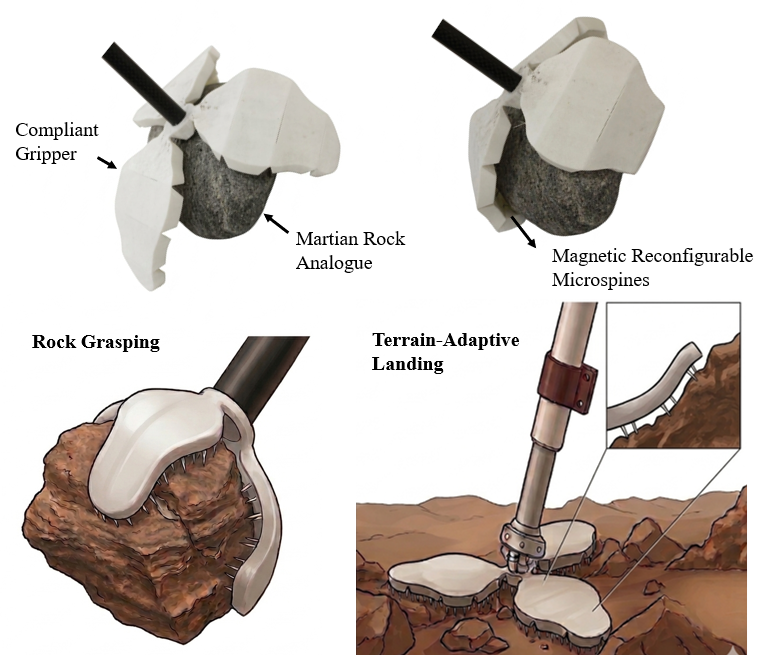
\includegraphics[width=.98\linewidth]{Picture1.png}
\caption{ Modular soft gripper with press-fit silicone microspine modules as a reconfigurable add-on end-effector, supporting (left) rock grasping and (right) terrain-adaptive landing from the same compliant structure. Modules enable tool-free spine swap while improving distributed asperity contact.}
\label{figure1}
\vspace{-3mm}
\end{figure}

Microspine-based attachment offers a promising strategy for such interactions. Microspines are small hook-like elements that engage with surface asperities and generate mechanical interlocking rather than relying on suction, magnetic adhesion, or chemical adhesives. This makes them attractive for dusty, porous, rocky, or irregular environments where conventional attachment methods are ineffective. Previous work has shown that compliant arrays of microspines can support climbing and attachment on hard rough surfaces by distributing loads over multiple individual contacts \cite{Asbeck2006IJRR,Kim2005SpinybotII,Spenko2008RiSE}. The same principle has also been explored for space-relevant anchoring, gravity-independent mobility, asteroid capture, and deep-ocean geological sampling \cite{Parness2012Microspines,Parness2013RockClimbing,Merriam2016AsteroidCapture,Parness2017ARM,Backus2020Nautilus}.

Soft robotic grippers provide complementary advantages for uncertain natural environments. Their compliance allows them to conform passively to irregular objects, distribute contact forces, and tolerate positioning errors during grasping \cite{Rus2015SoftRobotics,Shintake2018SoftGrippers}. These properties are particularly relevant for planetary manipulation, where rocks may vary widely in shape, size, roughness, and fragility. However, purely soft or friction-based grippers may struggle to generate sufficient attachment forces on hard, angular, dusty, or poorly envelopable rocks. Combining compliant gripper bodies with microspine arrays is therefore an attractive hybrid approach: the soft structure adapts to uncertain rock geometry, while the microspines provide local mechanical engagement with asperities. 

Despite these advantages, microspine attachment is sensitive to both surface characteristics and spine condition. Repeated contact with abrasive surfaces can cause tip blunting, plastic deformation, or fracture, reducing the ability of individual spines to engage surface asperities \cite{Underactuated_2023}. This challenge is particularly relevant to planetary exploration, where abrasive regolith particles common in space dust may contribute to the wear of exposed mechanical components \cite{Kalacska2024RegolithAbrasion}. Furthermore, spine geometry influences engagement with different surface textures, making a single fixed configuration unsuitable for all contact conditions \cite{Jiang2018StochasticSpines}. These limitations motivate a modular approach in which microspine arrays can be exchanged to accommodate different surface characteristics or replace damaged contact elements, without modifying the underlying gripper structure.

These considerations are particularly relevant to planetary exploration, where contact surfaces can vary substantially between geological environments. The Mars 2020 mission has identified diverse igneous, sedimentary, and aqueously altered materials within Jezero crater \cite{Farley2020Mars2020,Mangold2021JezeroDelta,Farley2022JezeroIgneous}. Differences in surface texture, asperity scale, and dust coverage may affect microspine engagement and the suitability of a particular spine configuration. A reconfigurable contact interface therefore offers a means of selecting different microspine morphologies for anticipated terrain conditions while retaining the same compliant gripper architecture.

Despite the maturity of microspine attachment and soft gripping as separate research areas, their combined use for Martian rock grasping and terrain-adaptive landing remains insufficiently understood. Existing studies have demonstrated impressive attachment forces and field capabilities on rough surfaces, but they often focus on a specific mechanism, a limited set of test surfaces, or applications such as climbing, asteroid anchoring, or underwater sampling. Although compliant microspine arrays and soft robotic grippers have been extensively investigated, microspine morphology is commonly determined during fabrication, limiting subsequent changes to the contact interface. Existing systems primarily address surface variability through passive compliance or predefined spine arrangements. In contrast, the present work investigates a modular contact interface that allows microspine geometry and distribution to be changed independently of the compliant gripper structure, while also enabling the replacement of worn or damaged modules.

%% Also talk about space grease! Especially for aplications in picking up space rocks!How does shape, smoothness, dust, or grease change this gripper interaction. First an investigation and showing how potentially, this could be applied via a reconfigurable setup. 

This paper investigates soft robotic grippers enhanced with reconfigurable microspine arrays for extraterrestrial rock grasping. We experimentally evaluate multiple gripper architectures and microspine configurations, varying parameters such as spine number, spatial distribution, orientation, and placement on compliant fingers or pads. The grippers are tested on Mars-relevant rock analogues selected to represent different surface textures and mechanical interaction regimes. Performance is quantified through pull-off force, shear resistance, grasp success rate, repeatability, and observed failure modes.

The main contributions of this work are threefold. First, we present a compliant, tendon-driven gripper incorporating magnetically interchangeable microspine modules, enabling contact morphology to be changed without modifying the underlying actuation or gripper structure. Second, we demonstrate the fabrication and interchangeability of modules with different spine geometries and distributions, providing a configurable contact interface that also permits replacement of worn or damaged elements. Third, we present preliminary rock-grasping results using selected microspine configurations, highlighting their potential for interaction with irregular geological surfaces and identifying limitations for future development.


\section{Related Work}

\subsection{Microspine attachment and passive adaption}

Microspine attachment was originally developed as a bio-inspired strategy for climbing and anchoring on hard rough surfaces, exploiting small-scale asperities to generate mechanical interlocking rather than relying on adhesion or suction (Fig.~2). Early work by Asbeck et al.\ demonstrated compliant microspine arrays enabling attachment on concrete, brick, and stone~\cite{Asbeck2006IJRR}, while SpinyBot and RiSE showed how directional spines and compliant suspensions can be integrated into legged climbing robots~\cite{Kim2005SpinybotII,Spenko2008RiSE}. These studies alongside others establish that microspine attachment depends on the relationship between spine tip geometry, surface asperity characteristics, and the compliance of the supporting structure \cite{Jiang2018StochasticSpines}. More recent underactuated microspine grippers have improved passive adaptation to uncertain contact conditions \cite{Li2023MicrospineGripper}. However, passive compliance primarily accommodates surface variations during interaction, rather than enabling the installed microspine morphology to be changed between tasks.

% Find work related to my sensors can work with this

\subsection{Microspines in space and field robotics}

Parness et al.\ developed gravity-independent mobility and drilling systems using hierarchical microspine arrays on vesicular basalt and a'a lava, demonstrating attachment under tangential, normal, and oblique loading~\cite{Parness2012Microspines}, later extended to rock-climbing robots and sample acquisition tools for low-gravity surfaces~\cite{Parness2013RockClimbing}. Microspine grasping has also been explored for asteroid capture~\cite{Merriam2016AsteroidCapture} and boulder anchoring in the context of the Asteroid Redirect Mission~\cite{Parness2017ARM}, where reliable attachment must be achieved without gravity-supplied preload --- a challenge shared by lightweight aerial or legged platforms operating on steep Martian terrain. In field robotics, the JPL-Nautilus gripper demonstrated effective grasping of irregular natural rocks for deep-ocean geological sampling~\cite{Backus2020Nautilus}, showing that microspines can perform outside idealised laboratory settings.
These studies demonstrate the potential of microspine attachment for geological sampling and robotic interaction with irregular natural surfaces. However, microspine geometry and arrangement are generally selected for the intended operating conditions, while variations in local surface geometry are accommodated through compliant mechanisms. For planetary exploration, where surface characteristics may vary considerably between locations such as on Mars with the olivine-rich cumulates of Jezero's Seitah unit or the fine-grained basalatic plains across Tharsis and Elysium, the ability to exchange microspine configurations could provide additional flexibility. Replaceable contact elements may also facilitate maintenance following abrasive wear or mechanical damage, without requiring replacement of the complete gripper. Despite this diversity, no prior work has systematically mapped microspine morphology to Martian rock types. Parness et al.\ demonstrated attachment on vesicular basalt and a'a lava~\cite{Parness2012Microspines} and the JPL-Nautilus gripper showed effective grasping on natural rocks~\cite{Backus2020Nautilus}, but neither addressed reconfigurability across surface types. This gap motivates the terrain-compatibility framework proposed in this paper.

\begin{figure*}
\centering
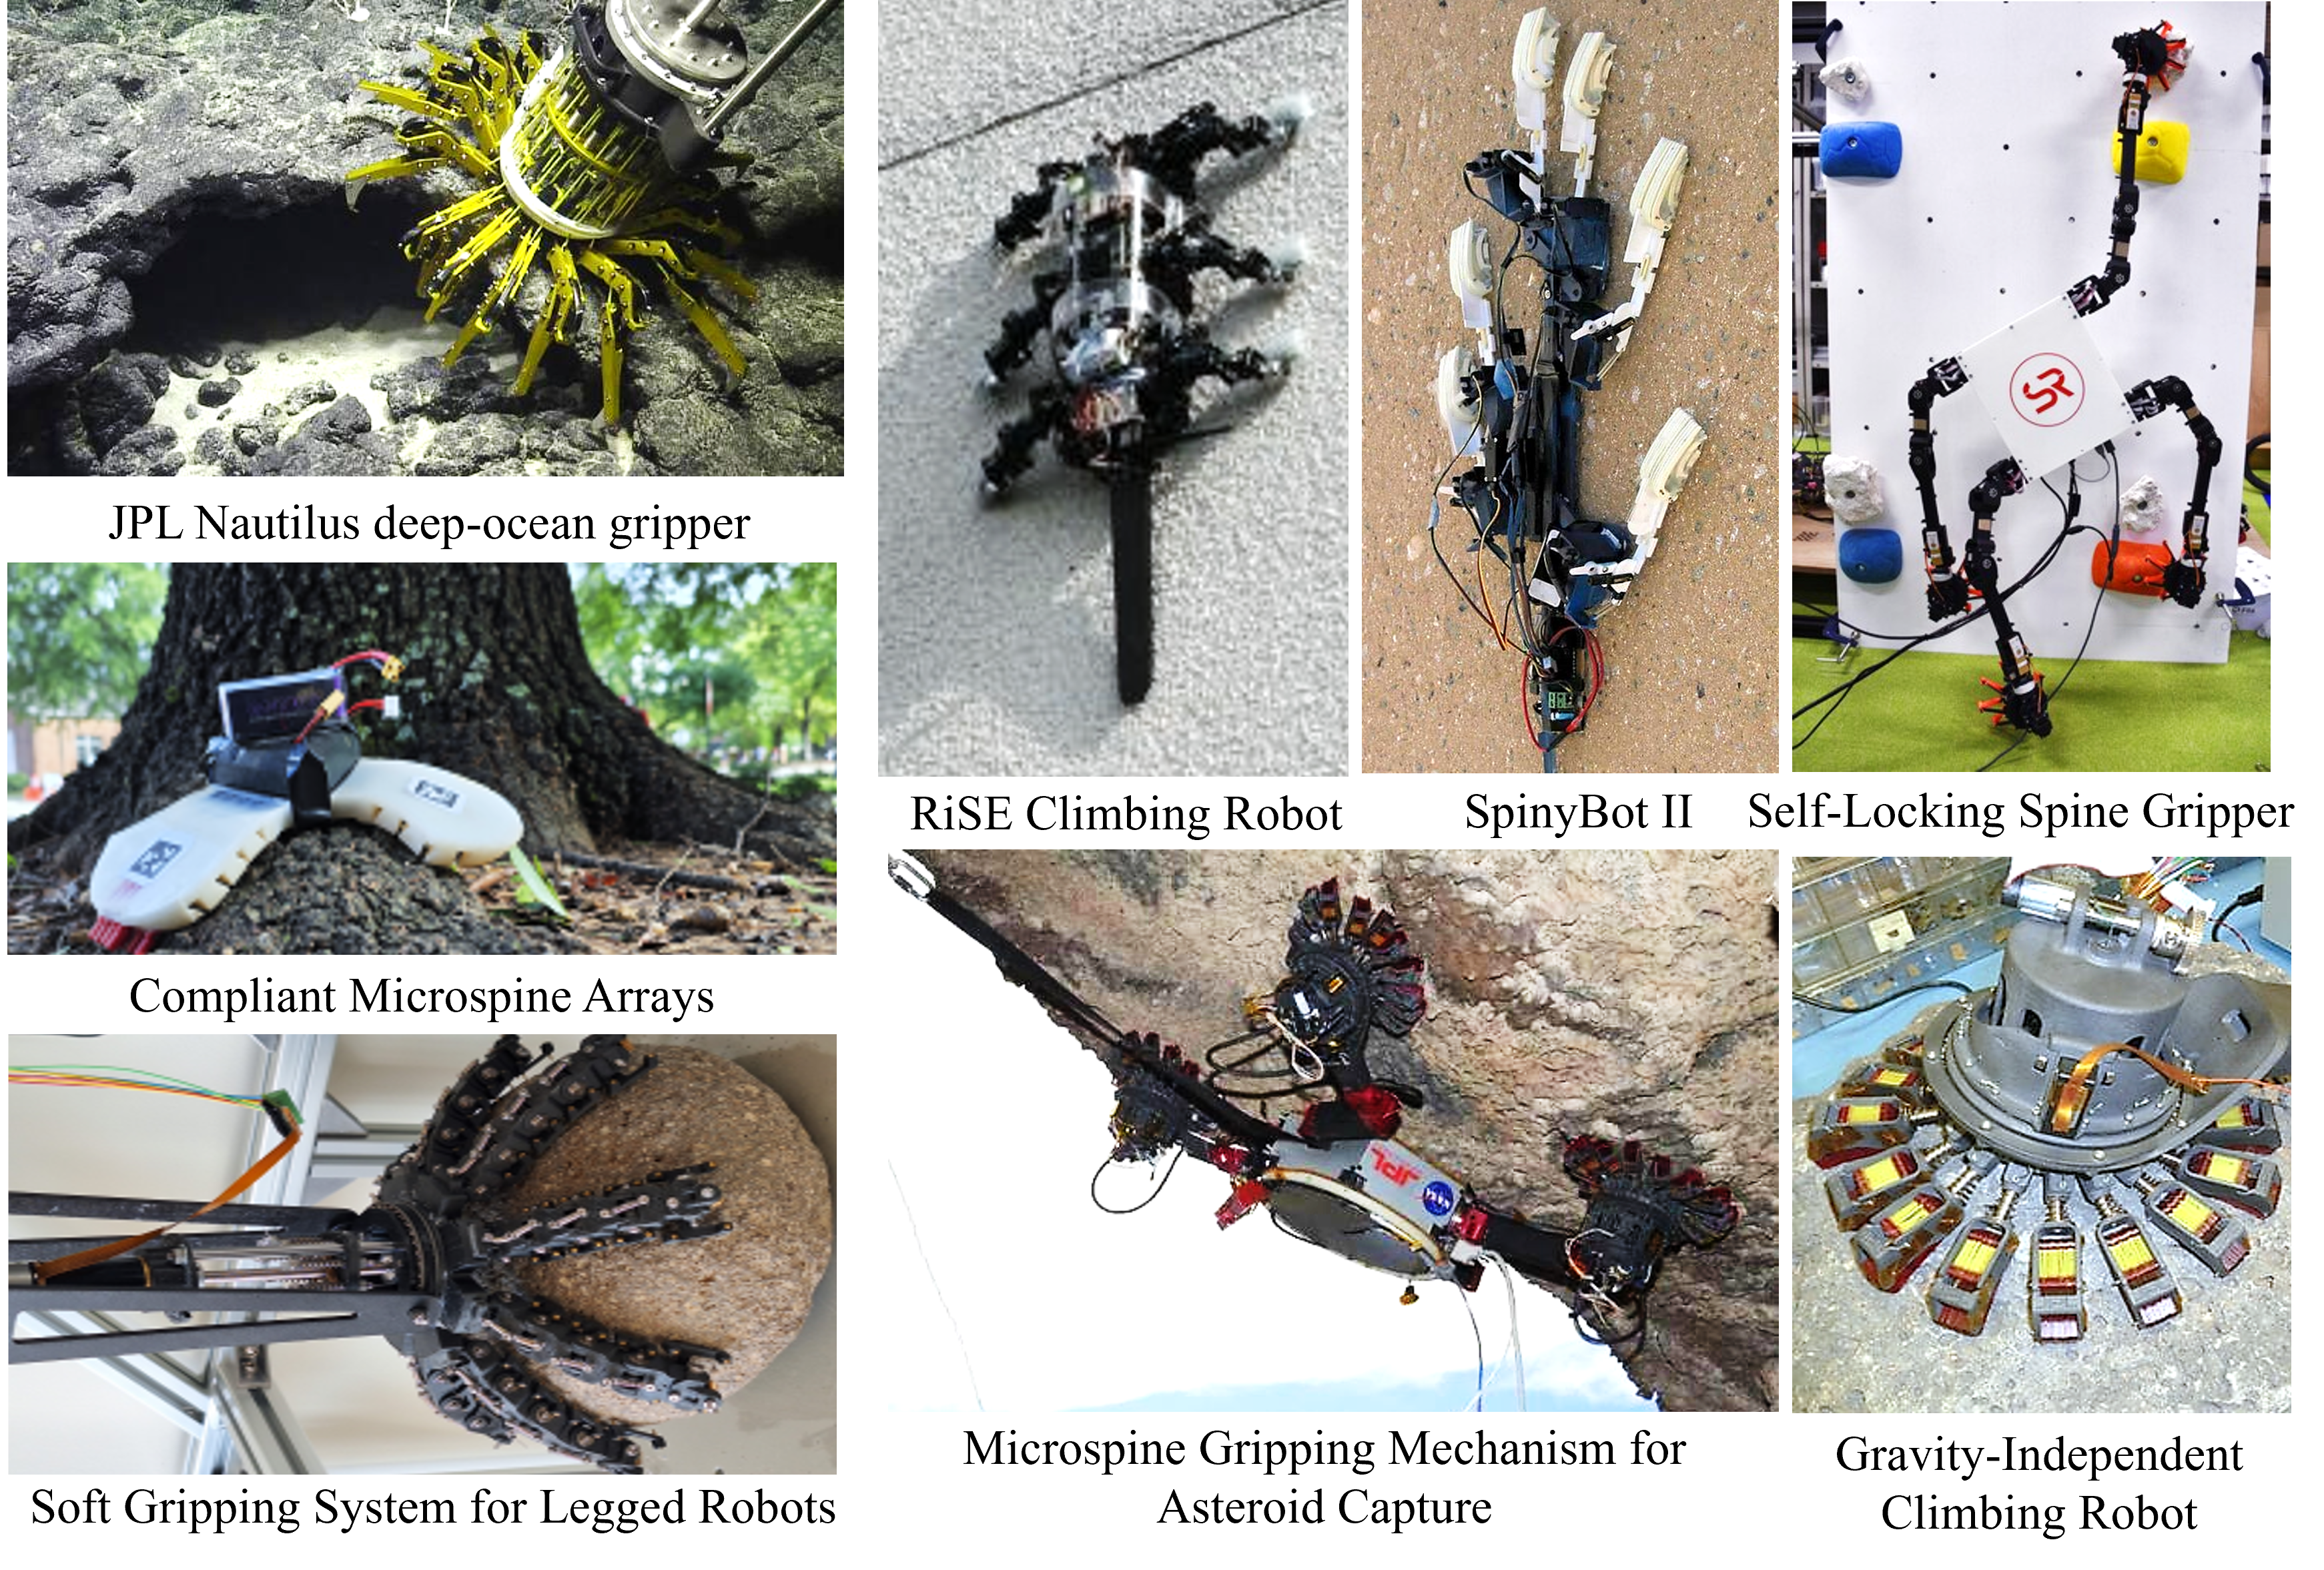
\includegraphics[width=.9\linewidth]{Picture7.png}
\caption{Representative microspine-based systems from the literature, illustrating the breadth of applications: deep-ocean geological sampling (JPL Nautilus gripper~\cite{Backus2020Nautilus}), rough-surface climbing (RiSE climbing robot~\cite{Spenko2008RiSE} and SpinyBot II~\cite{Kim2005SpinybotII}), tree-climbing and compliant array attachment~\cite{compliant_microspine_arrays}, low-gravity anchoring and mobility (JPL microspine grippers and gravity-independent climbing robot~\cite{Parness2013RockClimbing}), asteroid capture~\cite{Merriam2016AsteroidCapture}, self-locking attachment on vertical surfaces~\cite{Panorel02112025}, and soft gripping for space exploration legged robots \cite{candalot2024}. Despite their diversity of application, all existing systems share a common limitation: microspine morphology --- including spine thickness, density, and distribution --- is fixed at design time and cannot be reconfigured for different surface types or operational scenarios. This constrains their adaptability to the geological variability expected in Martian exploration, where a single platform may encounter basaltic outcrops, coarse-grained igneous rocks, pyroclastic deposits, and fluvially rounded cobbles within the same mission.}
\label{figure2}
\vspace{-3mm}
\end{figure*}



\subsection{Reconfigurable grippers and contact interfaces}

Soft robotic grippers offer passive adaptation to irregular objects through compliant structures, allowing them to accommodate variations in geometry and contact conditions \cite{Rus2015SoftRobotics,Shintake2018SoftGrippers}. However, structural compliance alone does not allow the contact properties of a gripper to be modified for different tasks. Recent work has investigated configurable microspine arrays for tendon-driven soft robots, demonstrating how alternative spine arrangements influence interaction with rough, unstructured terrain \cite{compliant_microspine_arrays}.

Reconfigurable grippers offer an alternative approach by enabling contact elements to be exchanged independently of the underlying robotic system. Ringwald et al. demonstrated automated production and exchange of task-specific fingertips for robotic manipulation \cite{Ringwald2023ModularFingers}. Similarly, Furia et al. developed interchangeable soft fingertips with different surface patterns to accommodate variations in agricultural grasping applications \cite{Furia2026GraspBerry}. Magnetically coupled modular soft fingers have also been investigated by Malik et al., enabling rapid exchange of pneumatic gripper configurations \cite{Malik2025ModularGripper}.

These studies demonstrate the benefits of interchangeable contact elements, ranging from complete soft fingers to task-specific fingertips. The present work extends this approach to microspine-based grasping of irregular geological surfaces, using magnetically interchangeable contact modules while retaining the compliant finger structure and tendon-driven actuation system. This enables changes in spine geometry and distribution without replacing the underlying finger or its actuation mechanism. Exchanging only the contact modules may also reduce the mass and volume of spare components required for reconfiguration and maintenance, an important consideration for mass-constrained planetary missions. Furthermore, worn or damaged microspine modules can be replaced without discarding the remaining finger structure.


\section{System Concept and Design Space}

The proposed system is a tendon-actuated soft robotic end-effector equipped with modular, interchangeable microspine arrays, designed as an add-on module for rock grasping on extraterrestrial locations such as Mars. The same compliant structure supports both use cases: in grasping mode, the three fingers close around a rock, conforming passively to its geometry while microspines engage surface asperities to resist pull-off and shear loads; in landing mode, the fingers act as compliant pads that anchor to rocky terrain by microspine interlocking, resisting shear forces and touchdown misalignment (Fig.~1).

\begin{figure}
\centering
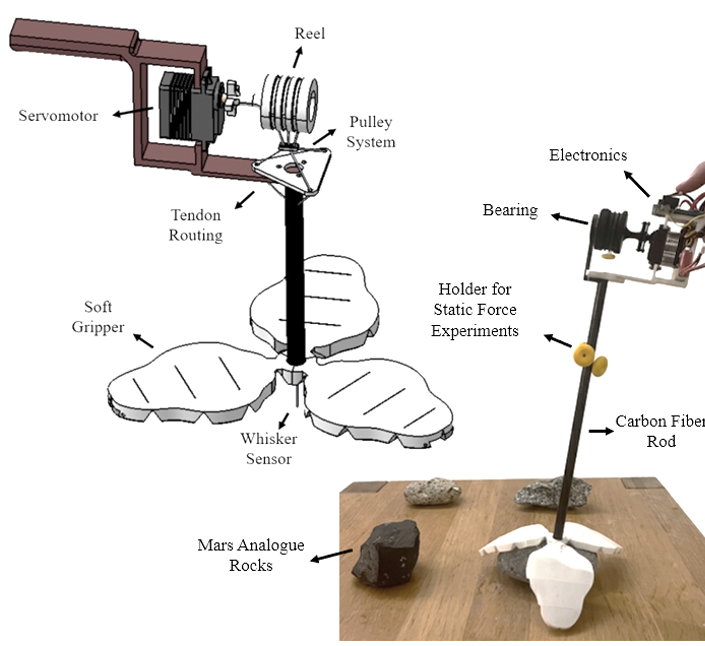
\includegraphics[width=\linewidth]{Picture5.png}
\caption{Tendon-actuated soft gripper system. Left: CAD model showing the servomotor-driven reel, pulley system, tendon routing, and integrated whisker sensor. Right: experimental setup showing the carbon fibre rod, bearing, electronics, and holder for static force experiments, with Mars analogue rocks.}
\label{figure3}
\vspace{-3mm}
\end{figure}

\begin{figure}
\centering
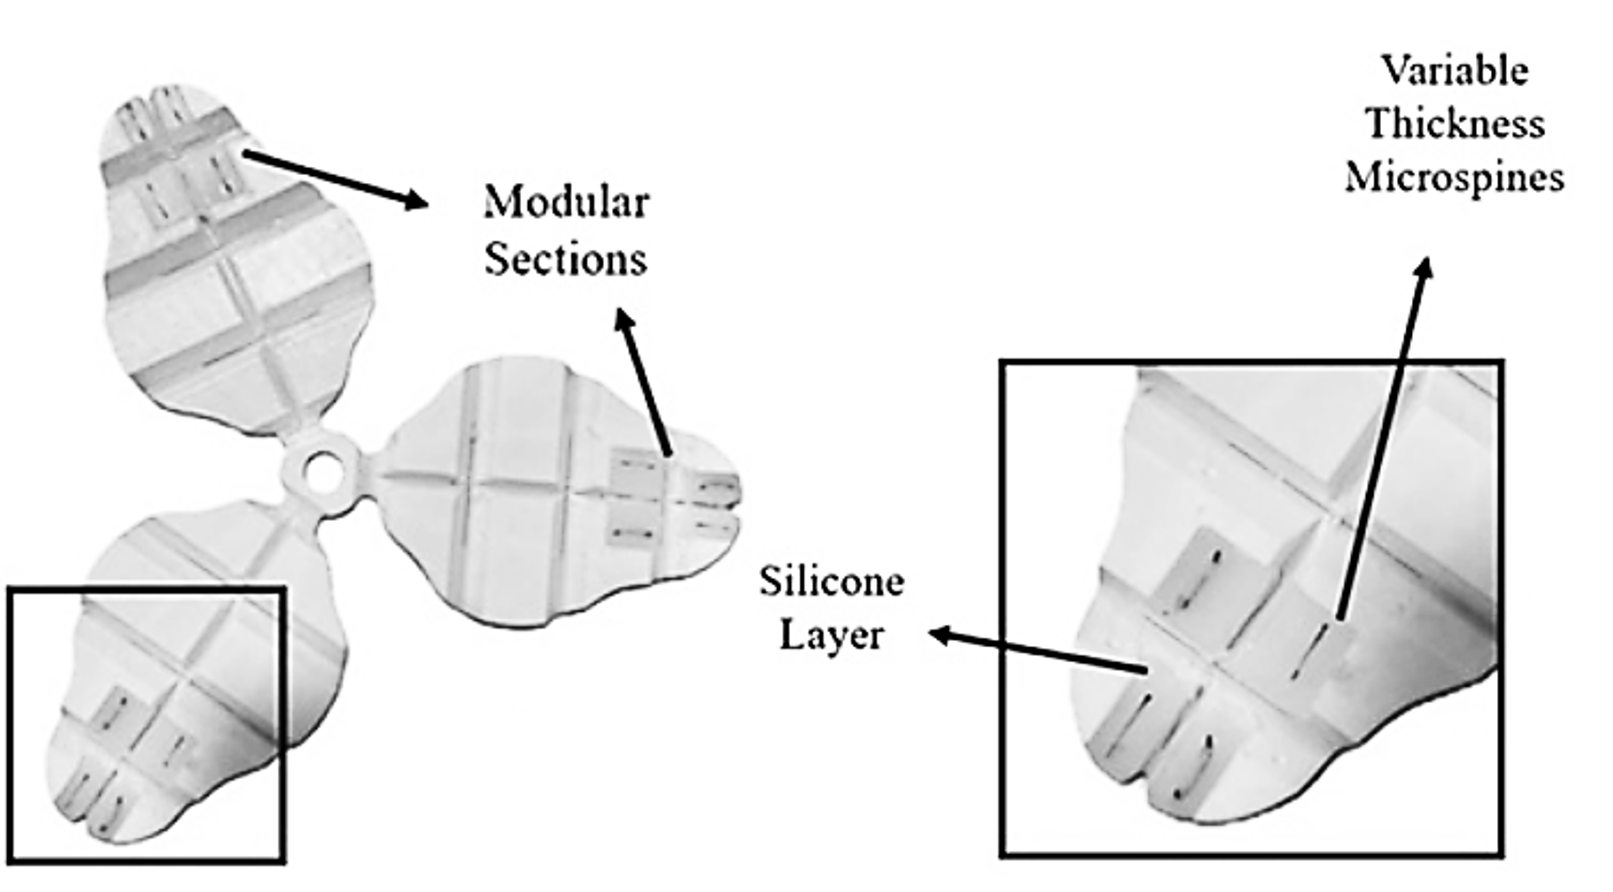
\includegraphics[width=\linewidth]{Picture4.png}
\caption{Fabricated gripper prototype with three modular finger sections. Each section accepts a press-fit silicone module embedding variable-thickness microspine arrays, enabling tool-free spine configuration swap without replacing the compliant TPU structure.}
\label{figure4}
\end{figure}

\begin{figure}
\centering
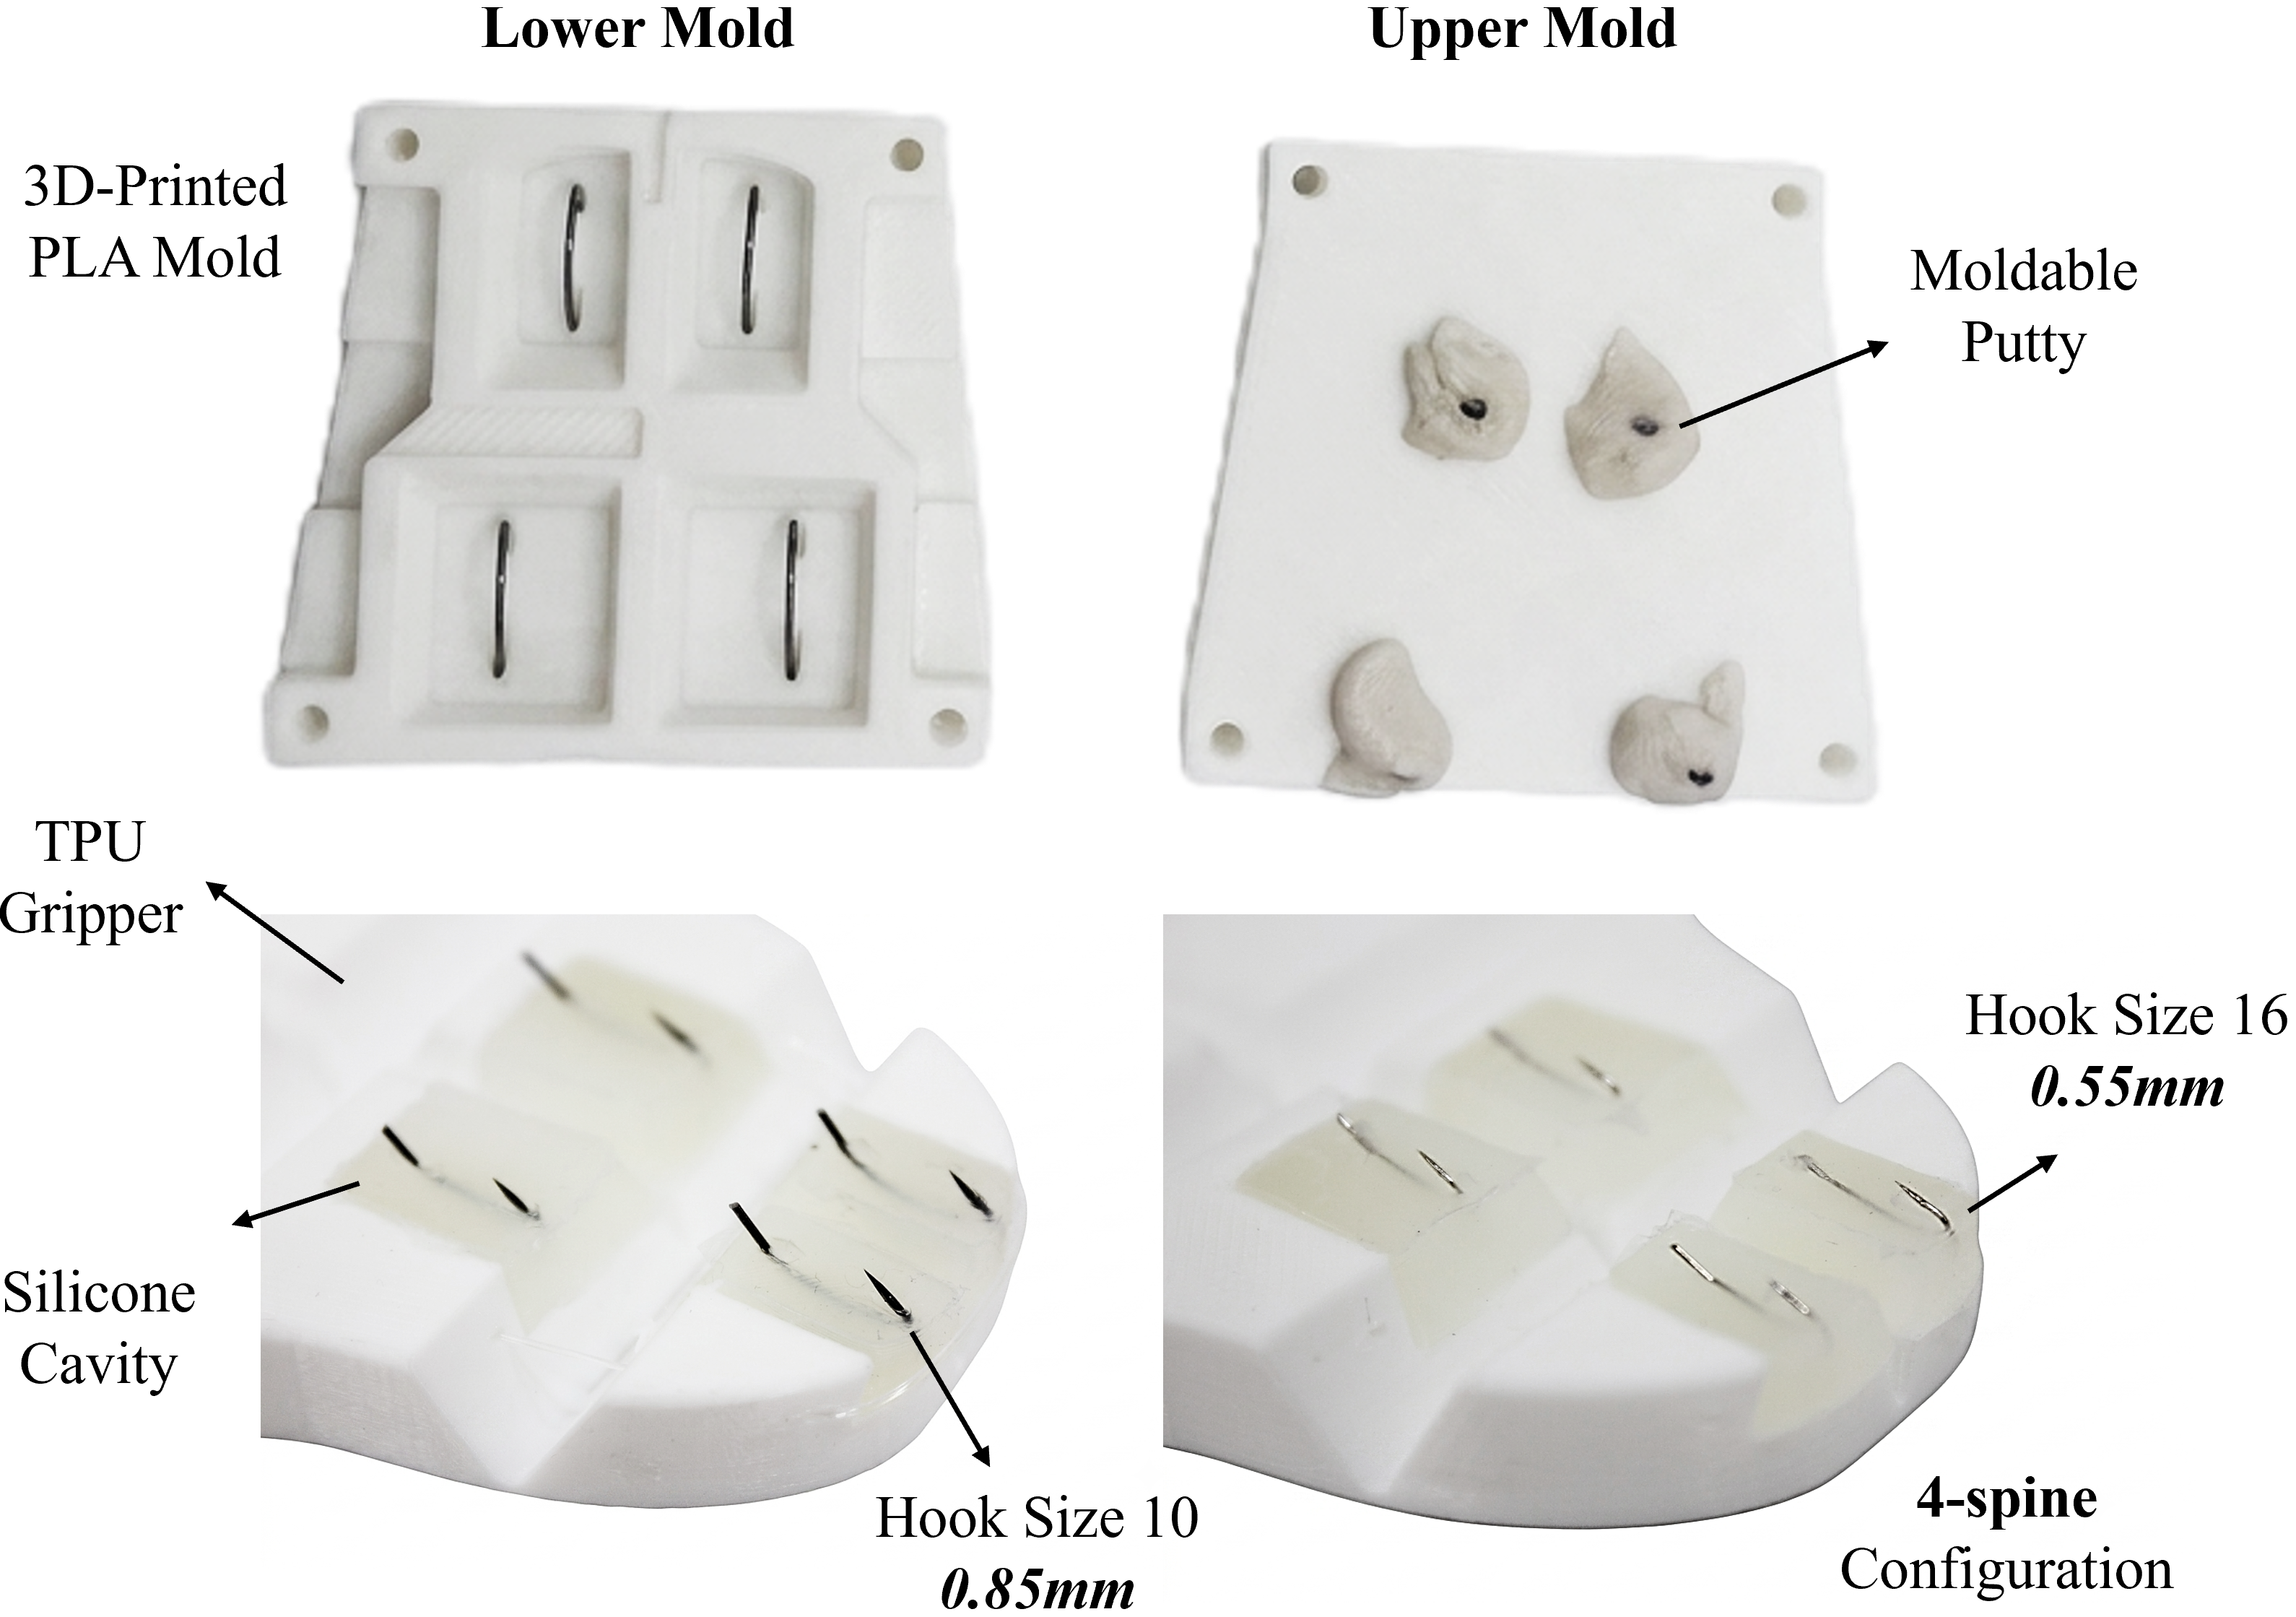
\includegraphics[width=\linewidth]{Picture2.png}
\caption{Microspine module fabrication. (top) Two-part PLA mold: lower half defines the silicone cavity and spine channels; upper half uses moldable putty to fix hooks at $\alpha=28$° prior to Ecoflex~0030 casting. (bottom) Fabricated modules press-fitted into the TPU finger, showing the silicone layer and two spine configurations: hook size~10 (0.85\,mm, thick-spine) and hook size~16 (0.55\,mm, thin-spine), both in a 4-spine arrangement.}
\label{figure5}
\vspace{-5mm}
\end{figure}

\subsection{Compliant Gripper Architecture}

\subsubsection{Finger Geometry and Magnetic Interface}

The gripper comprises a single compliant body with three fingers arranged at 120$^\circ$ intervals around its central mounting region. Each finger has nominal CAD dimensions of approximately 70\,mm in length, 35\,mm in width, and 8\,mm in thickness. The grippers and central hub were fabricated using Fused Deposition Modelling with TPU~95A filament on a Bambu Lab X1 Carbon printer (layer height 0.08 \,mm, and 15 \% infill). The compliant structure accommodates variations in object geometry, while the three-finger arrangement provides distributed contact around irregular rocks. Three fingers were selected as a compromise between grasp stability and system complexity, allowing independent finger actuation while limiting the number of motors, overall mass, power requirements, and control complexity.

Each finger incorporates four recessed mounting cavities, comprising two smaller front cavities and two larger rear cavities. The interchangeable microspine modules sit flush with the finger surface and are retained by two pairs of permanent N42 neodymium magnets, located along the side and base of each cavity. Each module contains two magnets of diameter 5\,mm and thickness 2\,mm. The corresponding finger magnets measure 5 $\times$ 2\,mm at the side and 10 $\times$ 2\,mm at the base, resulting in 24 embedded magnets across the three fingers.

The magnets are secured into closely fitted recesses with a strong adhesive. The cavity geometry provides repeatable positioning, while magnetic attraction retains the modules without mechanical latches. Modules can be removed manually by pulling or peeling from an edge, enabling tool-free replacement without modifying the compliant finger or actuation system.

\subsubsection{Actuation and Tendon Routing}

Each finger is independently actuated by a Feetech
HLS 2915M digital servo motor through a nylon fishing-line tendon. The tendons are wound onto 3D-printed PLA reels and routed through PTFE guides along the central
carbon-fibre shaft.

An initial open-gripper calibration establishes the required tendon travel. With the motors disengaged, the tendons are manually tensioned to define a reference configuration. During operation, a predefined motor-current threshold is used to stop further tendon retraction and limit excessive motor loading. This indirectly constrains grasp loading rather than providing direct control of the applied contact force.

\subsubsection{Sensors and Control}

A force-sensing resistor (FSR) is positioned between each interchangeable module and its corresponding finger cavity. Magnetic attachment compresses the FSR, providing a qualitative indication of module presence and changes in the sensor signal  also provide an indication of compressive contact loading on the module during a grasp.

A Teensy~4.0 microcontroller manages button-triggered gripper actuation and sensor data acquisition. The three Feetech servo motors are controlled through a URT-2 communication interface, with closure initiated by a button command. A configurable motor-current threshold provides a cut-off for further tendon retraction under excessive loading.


\subsection{Interchangeable Microspine Module Design
and Fabrication}

Microspine engagement on rough surfaces is inherently probabilistic, depending on the availability of suitable surface asperities and the ability of individual spines to establish and maintain mechanical contact. Engagement is influenced by spine tip geometry, orientation, loading direction, surface roughness, and the compliance of the supporting structure \cite{Jiang2018StochasticModels,Asbeck2006IJRR}. Consequently, different spine configurations may exhibit different attachment characteristics across natural surfaces. This motivates the development of interchangeable microspine modules, allowing spine size, number, and arrangement to be modified without changing the underlying gripper structure.

\subsubsection{Module Geometry and Spine Configurations}

The interchangeable contact modules are manufactured
from TPU~95A and incorporate embedded steel microspines formed from commercially available fishing hooks (Gamakatsu G-Code F314). The front two  modules are mirrored and measure approximately 9x7x15\,mm, while the rear two modules are also mirrored and measure approximately 13x7x16\,mm. Within each mounting location, the external module geometry and magnetic interface remain unchanged  to allow for easy modularity between spine configurations.

Several configurations were then fabricated to demonstrate interchangeability and explore variations in contact morphology. These include modules without spines, single- and double-spine arrangements using size-10 hooks, single-spine arrangements using larger size-6 or smaller size-18 hooks, and mixed-size arrangements. Where multiple spines are present, the hooks are predominantly positioned side by side to accommodate the limited module width. The measured wire diameters range from approximately 0.3\,mm for size-18 hooks to 0.8\,mm for size-6 hooks.


The selection of spine geometry is also influenced by the characteristics of the target rock surface. Larger, thicker spines are expected to be advantageous on coarse-grained igneous rocks such as dolerite, where prominent, mechanically stable asperities can provide engagement points for larger hooks. Conversely, smaller spines may be better suited to smoother surfaces, such as rounded ignimbrite cobbles, where finer asperities may be inaccessible to larger spine tips. Fine-grained basalt presents a further challenge due to the limited availability of suitable surface asperities, potentially reducing engagement across spine sizes. For weaker, clast-rich ignimbrite, engagement may instead be limited by local rock fracture, requiring consideration of the forces transmitted through individual spines. These contrasting surface characteristics motivate the use of interchangeable modules with different spine sizes and arrangements.

The number and arrangement of spines also influence attachment. Increasing spine number provides more potential engagement points across a rough surface, while reducing the number may allow individual spines greater freedom to accommodate local asperities. However, actual load sharing depends on the spatial distribution of contacts, spine compliance, and surface geometry \cite{Jiang2018StochasticModels}. The interchangeable modules therefore permit changes in spine size, number, and distribution without modifying the underlying gripper architecture.

Finally, spine orientation also influences asperity engagement, as the direction of applied loading relative to the local surface geometry affects whether an individual spine can establish stable contact \cite{Asbeck2006IJRR}. In the present design, the curved hooks are mounted at a nominal angle of approximately $40^\circ$ relative to the module contact surface. This angle is defined by the printed spine recesses, providing a consistent nominal orientation across configurations. The selected angle is treated as a fixed design parameter rather than an experimentally established optimum. The exposed lengths vary slightly with hook size, with approximately 1\,mm of the curved tip and 2\,mm of the trimmed shank protruding from the module.

%The gripper architectures are intentionally modular, allowing the same compliant body to be tested with different spine arrays. This enables a direct comparison between microspine configurations while reducing confounding effects from large changes in the gripper body. The modular design also reflects a possible future mission implementation, where end-effectors could be selected or optimized according to the expected terrain or sampling target.


\subsubsection{Embedded-Print Fabrication and Assembly}

The microspine modules were fabricated using fused
filament fabrication on a Bambu Lab X1 Carbon printer with TPU~95A filament, a 0.4\,mm nozzle, 0.08\,mm layer height, and 15\% infill. The modules were printed on their sides to allow the fishing hooks to be inserted horizontally during fabrication.

The print was paused at predefined layers corresponding to the insertion positions of the microspines. Before insertion, the hook eyes and portions of the shanks were removed. The hooks were then manually positioned in closely fitted recesses designed from their measured geometry. These recesses establish the nominal spine orientation without requiring an external positioning jig and keep the inserted hooks clear of the subsequent print-head path.

Printing was resumed after each insertion, encapsulating approximately 75\% of the hook within the TPU body, depending on the hook size. The surrounding material confines the embedded hook geometry, while the tip and a portion of the shank remain exposed. Following printing, the protruding shanks were trimmed to the required lengths, and the modules were visually inspected for hook alignment and printing defects.

No support structures were required. A wide first-layer brim was incorporated to improve bed adhesion and reduce the risk of module displacement during manual hook insertion. Finally, two N42 neodymium magnets (5\,mm diameter, 2\,mm thickness) were inserted into the open side and base recesses of each module and secured using a strong adhesive. The magnets were oriented to attract their corresponding counterparts in the finger cavities.


\subsection{Motor Mount and Assembly}

The motor mount and tendon reels were fabricated
from PLA (0.2\,mm layer height, 15\% infill) using a Bambu Lab X1 Carbon printer and houses the three Feetech HLS 2915M digital servo motors. Each motor drives a separate PLA reel (diameter 40\,mm). Nylon tendons are each wound onto this reel with a circumferential groove and redirected through a carbon fibre shaft (outer diameter 12\,mm). Three through-holes (diameter 2\,mm), one per finger, route the tendon along the shaft, where it splits into three branches fixed to the distal end of each finger. The motors are connected to a URT-2 bus communication board and controlled via the Arduino Teensy board. This board also allows the current readout from each digital motor to be read and separately controlled upon rock  contact.

\subsection{Mars-Relevant Rock Analogues}

Four natural rock specimens were selected to investigate microspine interaction with different surface geometries and textures. The specimens were geologically identified and comprise of dolerite, basalt, clast-rich ignimbrite, and a naturally rounded ignimbrite cobble (Table~\ref{tab:analogues}).

The selection encompasses coarse- and fine-grained igneous surfaces, heterogeneous clast-rich textures, and smooth, convex geometries. Surface characteristics were assessed qualitatively from geological knowledge and visual inspection rather than quantitative roughness or hardness measurements.

These specimens represent contrasting contact conditions relevant to planetary rock manipulation, rather than direct reproductions of specific Martian sites. Similar geological diversity has been observed during Mars exploration, including igneous and sedimentary materials in Jezero crater
\cite{Farley2022JezeroIgneous,Mangold2021JezeroDelta}. The differences in surface geometry and asperity characteristics provide a basis for investigating the potential benefits of interchangeable microspine configurations as explored further in Section~IV.

\begin{table}[t]
\caption{Mars-relevant rock analogues and microspine interaction}
\label{tab:analogues}
\centering
\footnotesize
\renewcommand{\arraystretch}{1.35}
\setlength{\tabcolsep}{5pt}
\begin{tabular}{p{1.8cm} p{2.8cm} p{3.2cm}}
\hline
\textbf{Sample} & \textbf{Martian occurrence} & \textbf{Microspine relevance} \\
\hline
Dolerite \newline {\scriptsize phaneritic, hard, stable asperities} &
S\'e\'itah/Jezero~\cite{Farley2022JezeroIgneous}; Valles Marineris; Nili Fossae &
Favorable for thick spines; high engagement probability; low fracture risk \\

Basalt \newline {\scriptsize aphanitic, very hard, smooth } &
Gusev~\cite{Squyres2004Spirit}; Syrtis Major; Tharsis; Elysium &
Poor thick-spine engagement on fresh faces; thin spines required\\

Ignimbrite \newline (clast-rich) \newline {\scriptsize heterogeneous hardness, friable } &
Medusae Fossae†~\cite{Mandt2008MFF}; Apollinaris Mons; Hadriacus/Tyrrhenus paterae &
High success rate but low payload; matrix fracture dominant failure mode \\

Ignimbrite \newline (cobble) \newline {\scriptsize fluvially rounded, smooth, convex} &
Gale/Hottah~\cite{Williams2013Hottah}; Jezero delta~\cite{Mangold2021JezeroDelta} &
Grasping dominated by finger enveloping; microspine contribution limited \\
\hline
\multicolumn{3}{l}{\scriptsize †Inferred from orbital data; not confirmed in situ.} \\
\hline
\end{tabular}
\vspace{-3mm}
\end{table}


% As per comments, moved preliminary estimate into system concept. Unsure exactly where this is supposed to fit

% \subsection{Preliminary Static Force Estimates}
% \textcolor{red}{\textbf{I WILL MOST LIKELY REMOVE THIS}}
% Direct measurement of static shear and pull-off forces in microspine-rock interaction is experimentally challenging: engagement forces vary significantly between trials due to the stochastic nature of asperity contact, and decoupling shear from normal components requires instrumentation not available at this stage. We therefore derive preliminary estimates by combining actuation system parameters with sustained payload measurements, and back-calculate $P_{eng}$ and $\bar{f}_{spine}$ across configurations and 
% rock types.

% The effective tendon force at the finger tip is $F_{eff} \approx 224$\,N. For the 4-spine configuration ($N_s = 4$), the estimated shear resistance per module is:
% %
% \begin{equation}
% F_{shear} \approx \mu \cdot F_{eff} = 0.3 \times 224 
% \approx 67\,\text{N}
% \end{equation}
% %
% and the mean engagement contribution per spine:
% %
% \begin{equation}
% P_{eng} \cdot \bar{f}_{spine} = \frac{F_{max}}{N_s}
% \end{equation}

%Table~\ref{tab:peng} summarises the estimated $P_{eng} \cdot \bar{f}_{spine}$ values per configuration and rock type, derived from sustained payload measurements and normalised engagement probability inferred from repeated trials.
%
% \begin{table}[h]
% \vspace{-3mm}
% \caption{Estimated $P_{eng} \cdot \bar{f}_{spine}$ 
% (N/spine) per configuration and rock analogue.}
% \label{tab:peng}
% \centering
% \footnotesize
% \renewcommand{\arraystretch}{1.3}
% \setlength{\tabcolsep}{4pt}
% \begin{tabular}{lcccc}
% \hline
% \textbf{Config.} & \textbf{Ign. clast} & \textbf{Dolerite} 
% & \textbf{Ign. cobble} & \textbf{Basalt} \\
% \hline
% Size 16 (thin)  & 0.67 & 0.30 & 0.64 & 0.15 \\
% Size 10 (thick) & 0.74 & 1.69 & 1.99 & 0.45 \\
% No spines       & 0.52 & 0.22 & 0.32 & 0.00 \\
% Mixed (10+16)   & 0.74 & 1.69 & 1.80 & 0.30 \\
% \hline
% \end{tabular}
% \vspace{-3mm}
% \end{table}

%Several observations follow. On dolerite and ignimbrite rounded cobble, the thick-spine configuration achieves the highest $P_{eng} \cdot \bar{f}_{spine}$, reflecting stable engagement with hard, well-defined asperities. On ignimbrite clast-rich, all spine configurations yield similar and relatively low values ($\approx$0.67--0.74\,N/spine), consistent with $\bar{f}_{spine}$ being limited by matrix fracture strength rather than spine geometry: engagement is achieved across configurations but load transfer is capped by surface failure. The mixed configuration approaches thick-spine performance on most surfaces while improving engagement on smooth geometries, suggesting broader terrain compatibility at the cost of reduced peak performance. Basalt yields the lowest values across all configurations, with thin spines and the baseline approaching zero, confirming that its aphanitic texture provides insufficient asperity scale for reliable engagement regardless of spine morphology. Full static characterisation will be reported in an extended version of this work.


\section{Experimental Results}

\subsection{Modular Interface Characterisation}

The retention of the magnetic modules was assessed
under nominally normal pull-off and tangential shear loading conditions until detachment from the finger cavity. The gripper was securely fixed, and an external load was applied exclusively to the selected module. The indicated load at the point of detachment was then recorded for each loading condition.

\begin{table}[t]
\caption{Force required for grip failure (gf), mean $\pm$ SD (sample SD, $n=5$ grasps per condition).}
\label{tab:spine_force}
\centering
\begin{tabular}{lccc}
\toprule
Object & No spines & 1 spine & 2 spines \\
\midrule
Smooth sphere & $200 \pm 54$   & $349 \pm 136$  & $320 \pm 76$ \\
Coarse sphere & $253 \pm 25$   & $832 \pm 202$  & $1040 \pm 201$ \\
Polyhedron    & $1010 \pm 182$ & $2076 \pm 278$ & $2658 \pm 1015^{\dagger}$ \\
\bottomrule
\multicolumn{4}{l}{\footnotesize $^{\dagger}$In 2 of 5 grasps a module detached at 1600 and 1500~gf;}\\
\multicolumn{4}{l}{\footnotesize the other three failed at $3397 \pm 117$~gf.}
\end{tabular}
\end{table}

Each loading condition was repeated ten times at two different mounting locations for both the front and rear module geometries, resulting in 80 trials. Detachment generally occurred at an indicated load of approximately 300\,gf (2.9\,N), with normal pull-off tending to occur slightly below this value and tangential shear loading slightly above it. Detachment was typically initiated through peeling at one edge with similar behaviour observed across the tested module locations.

These measurements characterise the retention of individual magnetic module-to-finger interfaces,
rather than the overall microspine grasping capacity as not all of the modules will necessarily engage the rock simultaneously. Furthermore, the loading direction and force distribution between the modules depend on the object geometry and contact conditions. Consequently, the individual detachment forces cannot be directly summed to estimate the maximum grasping force.

An additional characteristic of the magnetic interface is its potential to permit limited module displacement before complete detachment. This may allow passive redistribution of contact forces between neighbouring modules, while magnetic attraction could facilitate re-seating of partially displaced modules when the load is reduced. However, these mechanisms have not yet been experimentally characterised.


\subsection{Grasping Tests}
\subsubsection{Grasping Tests on Controlled Objects}

To establish a quantitative benchmark for the effects of surface texture and object geometry, the grasping capability of the gripper was evaluated using three objects: a smooth sphere, a coarse-textured sphere, and a rough polyhedron. Three interchangeable module configurations were investigated, incorporating zero, one, or two microspines per module. Each combination was evaluated over five trials under similar conditions, with the indicated load at grasp failure recorded.

\begin{figure*}[t]
\centering
\includegraphics[width=\textwidth]
{controlled_grasp_figure_two_column.pdf}
\caption{Indicated grasp-retention loads for
three test objects and three microspine
configurations ($N=5$ trials per condition).
Circles represent individual trials, diamonds
indicate the mean, and error bars show one
sample standard deviation. Triangles identify
trials terminated by magnetic module
detachment. Different vertical scales are
used for each object.}
\label{fig:controlled_grasping}
\end{figure*}

As shown in Tab.~\ref{tab:controlled_grasping}, the microspine configurations exhibited different retention characteristics across the test objects. For the smooth sphere, the mean indicated load increased from 1.96\,N without spines to 3.42\,N and 3.14\,N for the single- and double-spine configurations, respectively.

The effect was more pronounced on the coarse-textured sphere, for which the mean load increased from 2.48\,N without spines to 8.16\,N with one spine and 10.20\,N with two spines per module. Variation between trials was observed, consistent with differences in the local surface features encountered during contact. 

The highest loads were recorded on the polyhedron, reaching mean values of 9.90\,N, 20.36\,N, and 26.07\,N for the zero-, one-, and two-spine configurations, respectively. In the two-spine configuration, two of the five trials terminated through magnetic module detachment at approximately 14.7--15.7\,N, whereas the remaining three trials reached 32.1--34.3\,N. 

Several observations can be made from these tests. First that the surface finish of the objects grasped has a large  tests These failures indicate that while the shape of an object can provide the best gripping force, there is also a chance that the shape will load to failure one of the magnetic interfaces on the modules. Although the results demonstrate an increase in retention with the addition of microspines for the coarse sphere
and polyhedron, the small sample size
and variations in local engagement
limit broader conclusions regarding
optimal spine configurations.

\subsubsection{Grasping Tests on Natural Rocks} 

Grasping performance was evaluated using the four natural rock specimens described in Section~III.D. A trial was considered successful when the object could be lifted by 300\,mm and retained for 5\,s. A representative example of this testing is shown in Figure \ref{figure7_grasping_experiment}.

\begin{figure}
\centering
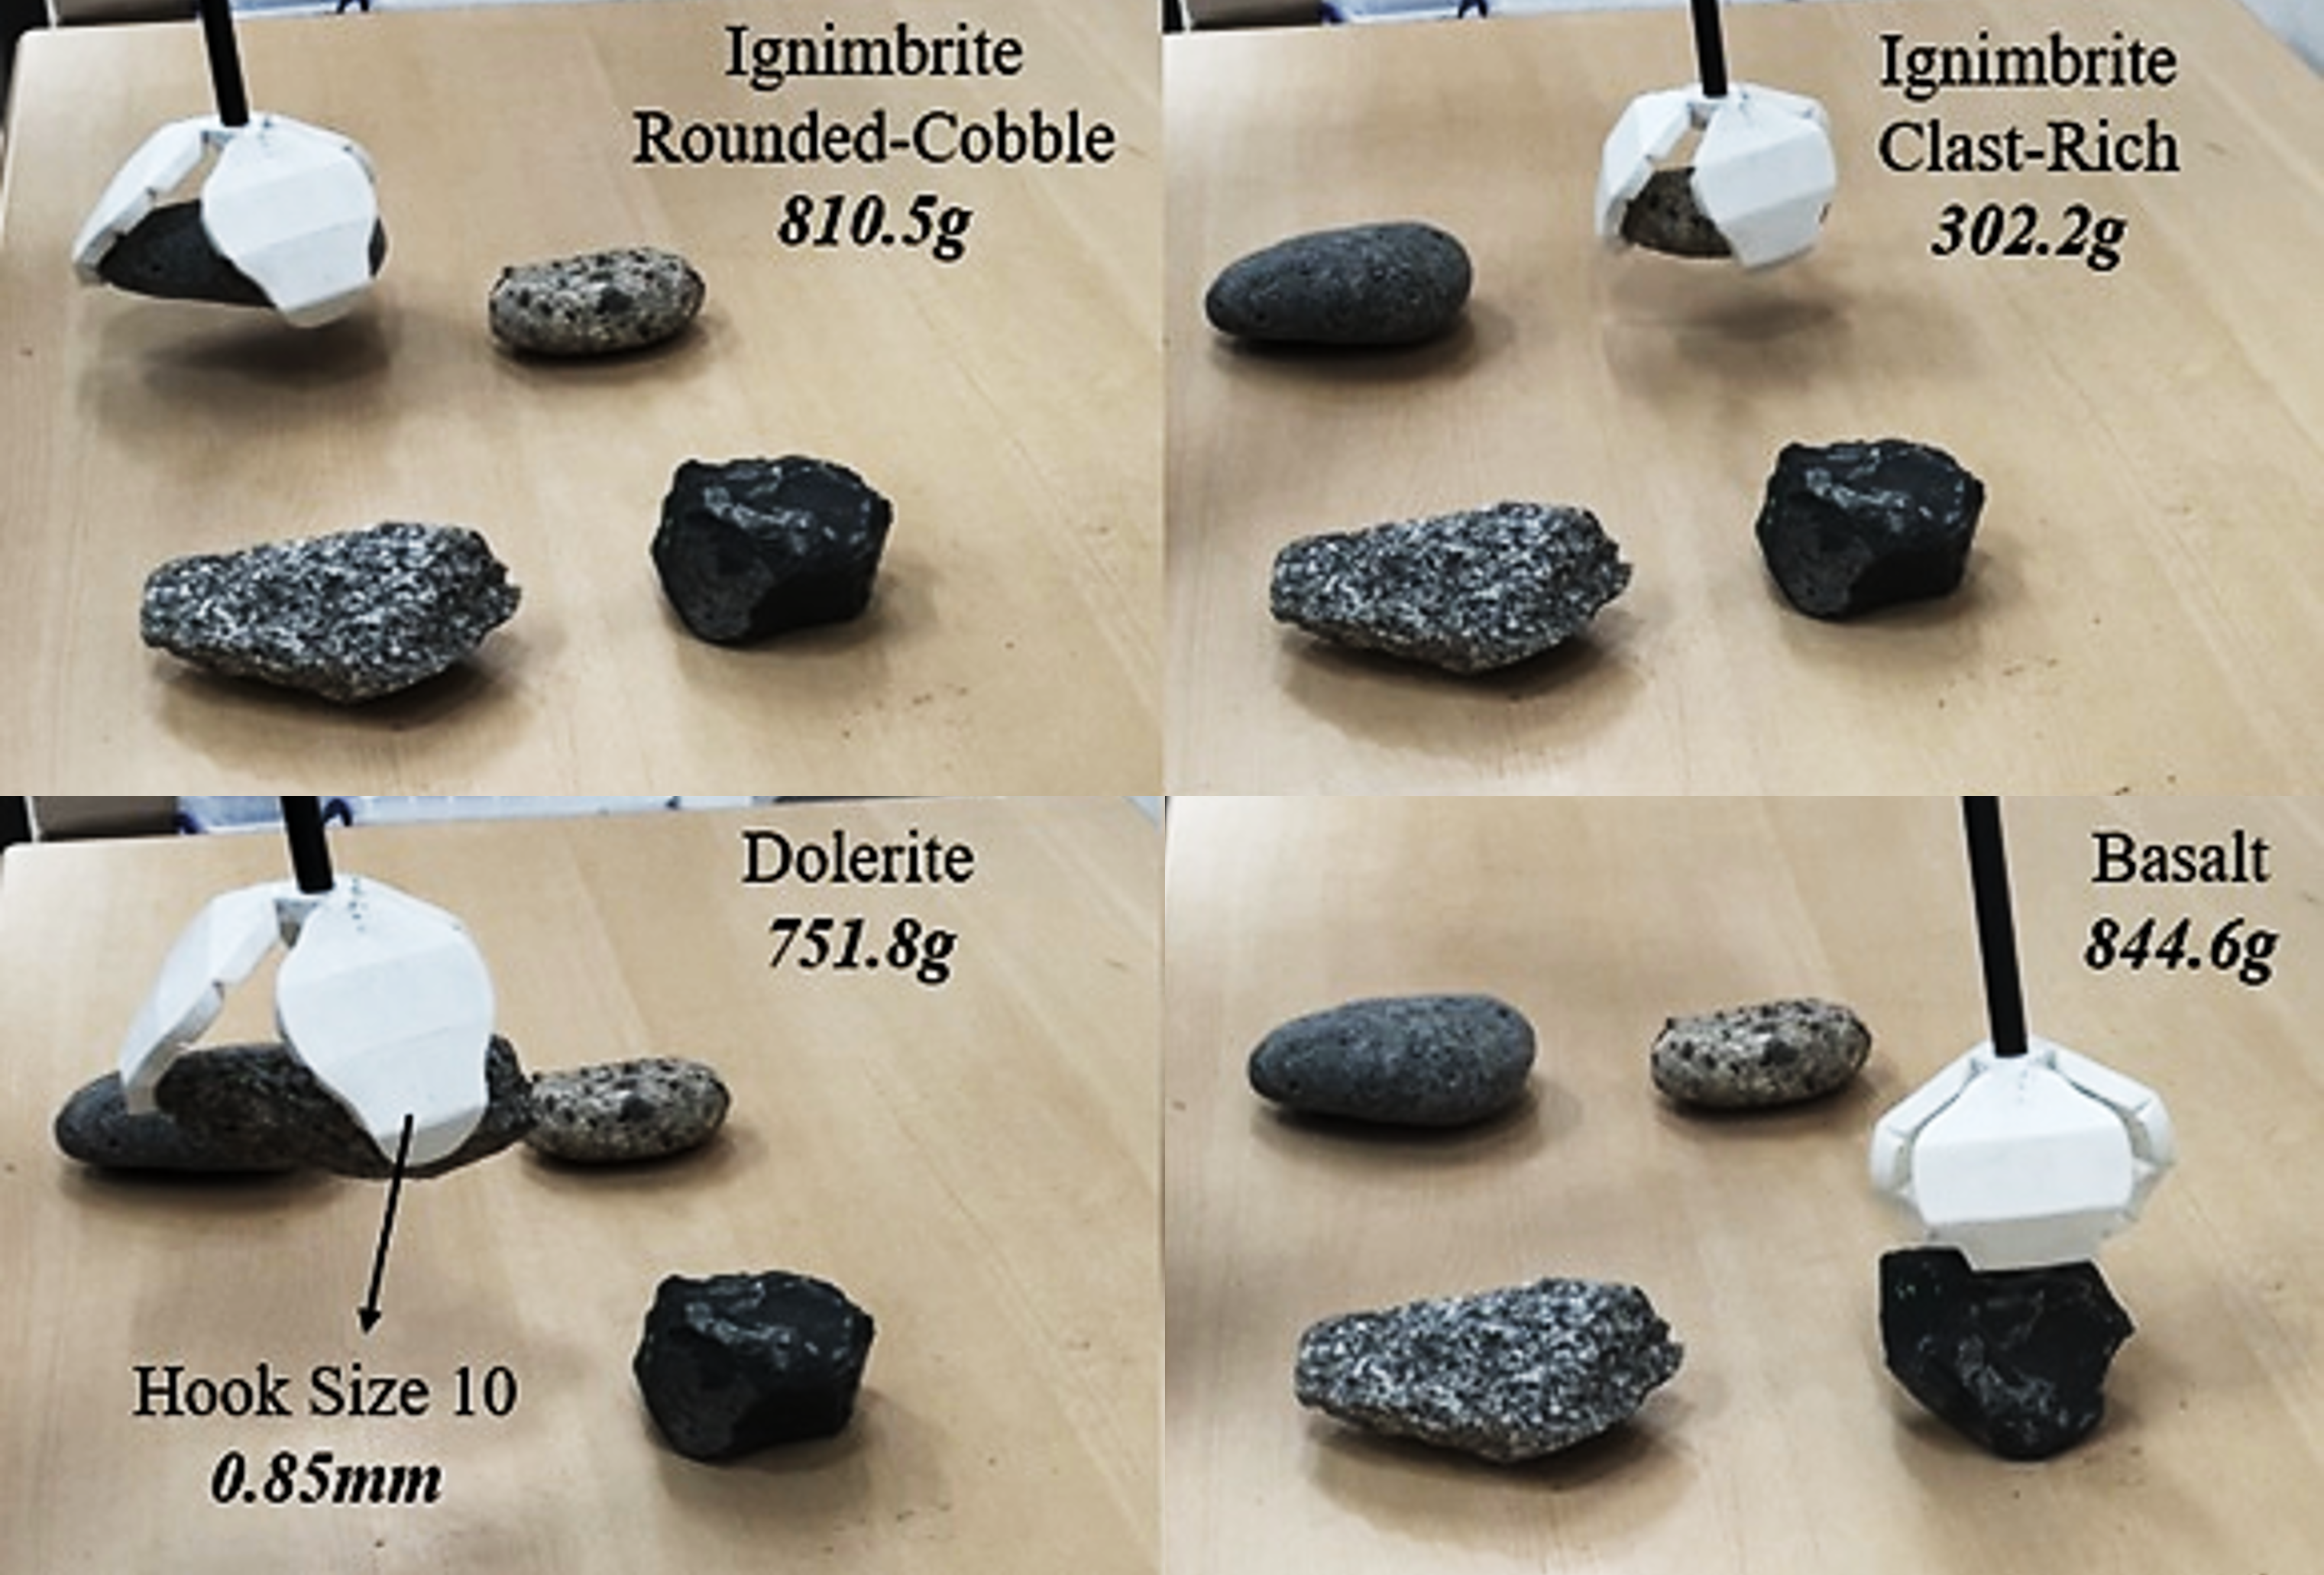
\includegraphics[width=\linewidth]{Picture6.png}
\caption{Grasping performance of the thick-spine configuration (hook size 10, 0.85mm) across the four Mars-relevant rock analogues, showing maximum sustained payload.}
\label{figure7_grasping_experiment}
\vspace{-3mm}
\end{figure}


Four configurations were investigated: thin spines (size~16), thick spines (size~10), no spines, and a mixed size-10/16 arrangement. Each configuration was tested ten times on each rock specimen, with the observed grasp success rates presented in Table~\ref{tab:grasping}.

\vspace{-3mm}
\begin{table}[h]
\caption{Observed grasp success rate (\%) per configuration and rock analogue.}
\label{tab:grasping}
\centering
\footnotesize
\renewcommand{\arraystretch}{1.3}
\setlength{\tabcolsep}{4pt}
\begin{tabular}{lcccc}
\hline
\textbf{Configuration} & \textbf{Ign. clast} & \textbf{Dolerite} & \textbf{Ign. cobble} & \textbf{Basalt} \\
\hline
Size 16 (thin)   & 90 & 40 & 80 & 20 \\
Size 10 (thick)  & 100 & 90 & 40 & 60 \\
No spines        & 70 & 30 & 40 & 0  \\
Mixed (10+16)    & 100 & 90 & 90 & 40 \\
\hline
\end{tabular}
\vspace{-3mm}
\end{table}


Several trends emerge from the results. First, the thick-spine configuration (size~10) outperforms thin spines on dolerite (90\% vs.\ 40\%), consistent with its coarse surface texture providing asperities suitable for engagement by larger hooks. Conversely, thin spines (size~16) achieve higher success on the rounded ignimbrite cobble (80\% vs.\ 40\%), where the relatively smooth, convex surface may favour engagement by smaller, more compliant spines. This inversion suggests that spine geometry influences engagement across different surface conditions, supporting the motivation for terrain-dependent microspine reconfiguration.


The mixed configuration (size~10+16) achieves the highest or equal success rate across three of the four rock specimens, notably reaching 90\% on the rounded ignimbrite cobble, where neither individual configuration exceeds 80\%. This suggests that combining spine sizes may improve the range of surface features accessible for engagement. The mixed arrangement therefore provides promising performance across the tested specimens, although its effectiveness on other surfaces remains to be established.

The baseline configuration without spines achieves 70\% success on clast-rich ignimbrite, indicating that compliant contact alone can provide sufficient retention under some conditions. However, it achieves no successful grasps on basalt, where the thick-spine configuration reaches 60\%. Basalt also produces the lowest success rates for the thin-spine and mixed configurations. These observations are consistent with the limited accessible asperities expected on relatively smooth, fine-grained surfaces, although the effects of specimen geometry and mass cannot be excluded.


As noted in Figure \ref{figure7_grasping_experiment}, the tested rock specimens ranged in mass from approximately 300 to 850\,g, with retention of heavier specimens generally less reliable. Observed grasp failures were associated with microspine slip, while the magnetic modules remained attached to their finger cavities.


\subsection{Terrain Compatibility Framework}
The grasping results and preliminary force estimates allow 
a first terrain-compatibility mapping between microspine 
configuration and Martian geological context 
(Fig.~7). The key finding is that no single 
spine configuration performs optimally across all rock types, 
which directly motivates the reconfigurable modular design 
proposed in this work.

Thick spines (size~10) are best suited for coarse-grained, 
high-asperity surfaces such as dolerite, representative of 
exhumed intrusive units at S\'e\'itah/Jezero, Valles 
Marineris, and Nili Fossae. Thin spines (size~16) are 
preferable on smooth convex surfaces such as ignimbrite 
rounded cobbles, confirmed at Gale and Jezero's western 
delta --- high-priority targets for Mars Sample Return. 
On ignimbrite clast-rich surfaces, inferred at Medusae 
Fossae and the highland paterae, all spine configurations 
achieve reliable engagement, but payload is limited by 
matrix fracture rather than spine morphology, suggesting 
that preload control is more critical than spine selection 
in this regime. Basalt, the globally dominant lithology 
across Tharsis, Elysium, and Syrtis Major, remains the 
most challenging surface for all configurations tested, 
with the mixed (10+16) configuration offering the best 
compromise.

The mixed configuration emerges as the most robust 
default for unknown terrain, combining the engagement 
range of both spine sizes at the cost of reduced peak 
performance on specialised surfaces. These results 
suggest that a two-module system --- thick for igneous 
outcrops, thin for fluvial or smooth surfaces --- would 
cover the majority of Martian geological scenarios 
identified in Fig.~7, with the mixed 
configuration as a fallback when surface type cannot 
be determined in advance.

\section{Conclusions}

This paper presented a compliant soft robotic gripper incorporating interchangeable microspine modules for extraterrestrial rock grasping. The magnetic attachment interface enables tool-free reconfiguration of spine geometry and distribution without modifying the underlying gripper structure. This provides a means of adapting the contact interface to different surface conditions and replacing worn or damaged microspines.

Preliminary grasping experiments across four Mars-relevant rock analogues demonstrated variations in grasping performance between microspine configurations, highlighting the influence of surface characteristics on mechanical engagement. The modular interface was additionally characterised through normal pull-off and shear detachment measurements of approximately 2.94 N, providing an initial assessment of module retention.

Future work will investigate individual motor-current calibration for more precise grasp-force regulation, automated module exchange, and validation under Mars-relevant environmental conditions, including dust and reduced gravity.

\begin{figure}
\centering
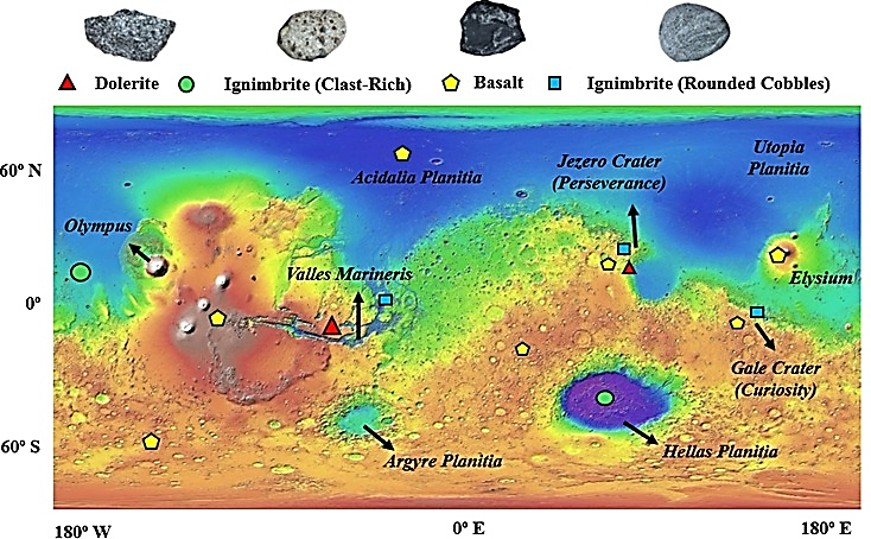
\includegraphics[width=.99\linewidth]{Picture3.jpg}
\caption{Martian occurrences of the four rock analogues on the MOLA topographic map (NASA/GSFC): dolerite (red triangle), basalt (yellow pentagon), ignimbrite clast-rich (green circle), ignimbrite rounded cobbles (blue square). Inset: experimental rock samples. Ignimbrite occurrences inferred from orbital data; all others confirmed in situ (Perseverance, Curiosity, Spirit).}
\label{figure5}
\vspace{-5mm}
\end{figure}


\bibliographystyle{IEEEtran}
\bibliography{IEEEabrv,References}
\end{document}